
\section{Design}

This section will detail the design of each of the main elements of the application; this includes: how the application is interacted with, how data is stored, and the services being ran.

\subsection{API}

This application should provide a set of HTTP endpoints that allow users to perform various CRUD operations. This includes:

\begin{itemize}
    \item creating and managing a set of devices that can be woken up using Wake-on-LAN,
    \item creating and managing recurring schedules for these devices to be woken up at,
    \item creating and managing a set of devices that can be watched by the application in order to trigger devices to be woken,
    \item create mappings between watched devices and devices that can be woken, and
    \item managing a set of background services that are used to track watched devices and environmental factors.
\end{itemize}

\subsection{Services}\label{subsec:services}

This section will describe the background services that are used to detect various conditions that when satisfied will trigger a set of devices to wake up. 

\vspace{2mm}
\subsubsection{Schedules}

This service will allow users to set recurring periods of time every week that a device should be woken up. Each schedule will detail:

\begin{itemize}[noitemsep]
    \item what device should be woken up,
    \item what day and time every week it should be woken up, and
    \item whether or not that schedule is active at this point in time.
\end{itemize}

\vspace{2mm}
\subsubsection{Scanning the LAN}

This service will periodically look for a \textit{watcher} device on the local network by sending an ARP request to it and seeing if a response is received. An example use case for this would have a user setting their mobile device as a watcher so when they join their home network all of their devices will be woken up.

\begin{figure}[H]
    \centering
    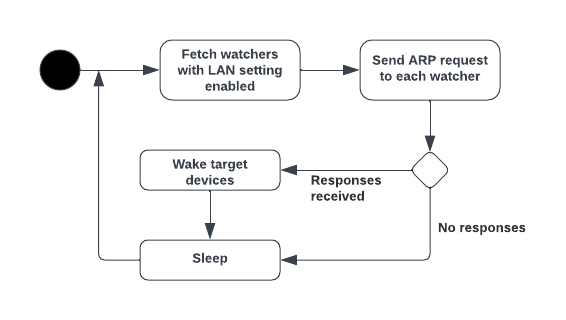
\includegraphics[width=\columnwidth]{assets/lan.png}
    \caption{A state diagram showing how devices are searched for on the LAN}
    \label{fig:my_label}
\end{figure}

Watcher devices will be checked for at regular intervals until they are discovered, and once they are found they will not be checked for again for a period of time specified by the user. This service will add extra congestion to the local network and relies on a device having a static IP address; most routers will use DHCP so users will have to set this manually. 

\vspace{2mm}
\subsubsection{Bluetooth}

 By allowing this application to search for Bluetooth devices, it increases the number of devices we can search for and removes the requirement from the previous section of being in the same LAN. On top of this, the watched device is referred to by its unique Bluetooth MAC address, which will never change, as opposed to a device's IP address, which will likely be allocated using DHCP and may change.

\begin{figure}[H]
    \centering
    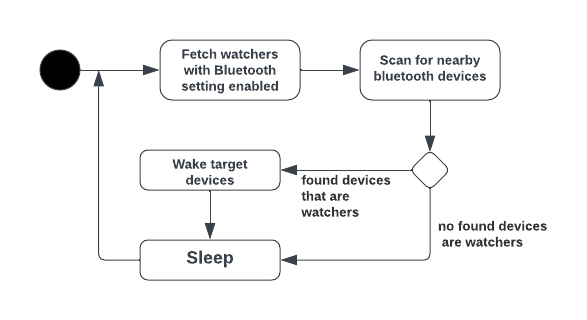
\includegraphics[width=\columnwidth]{assets/bluetooth.png}
    \caption{A state diagram showing how devices are searched for using Bluetooth}
    \label{fig:my_label}
\end{figure}


\vspace{2mm}
\subsubsection{Sniffing Traffic}

This service will sniff for packets being sent to a watcher device and if the packet meets a given set of conditions then we will wake a target device. An example use case for this would be a user remotely connecting to a home server and then having the application wake up any auxiliary servers, such as a file server. 

\begin{figure}[H]
    \centering
    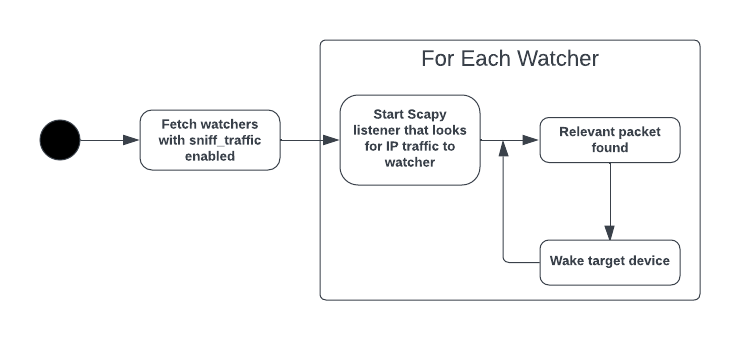
\includegraphics[width=\columnwidth]{assets/sniffer.png}
    \caption{A state diagram showing how devices are searched for using LAN packet sniffing}
    \label{fig:my_label}
\end{figure}

\vspace{2mm}
\subsubsection{Environment Sensors}

This application will have a set of services that use external sensors to consider various environmental factors; specifically: light, sound, and motion. The user will be able to set threshold values for each, such that when the sensor records a value that is above or below it a target device is woken up.

\subsection{Arc}

Figure~\ref{fig:architecture} shows a sample architecture for the application; where the user is accessing the API remotely over the internet. A watcher device joins the network, is detected, and the application then wakes up a different device.

\begin{figure}[ht]
    \centering
    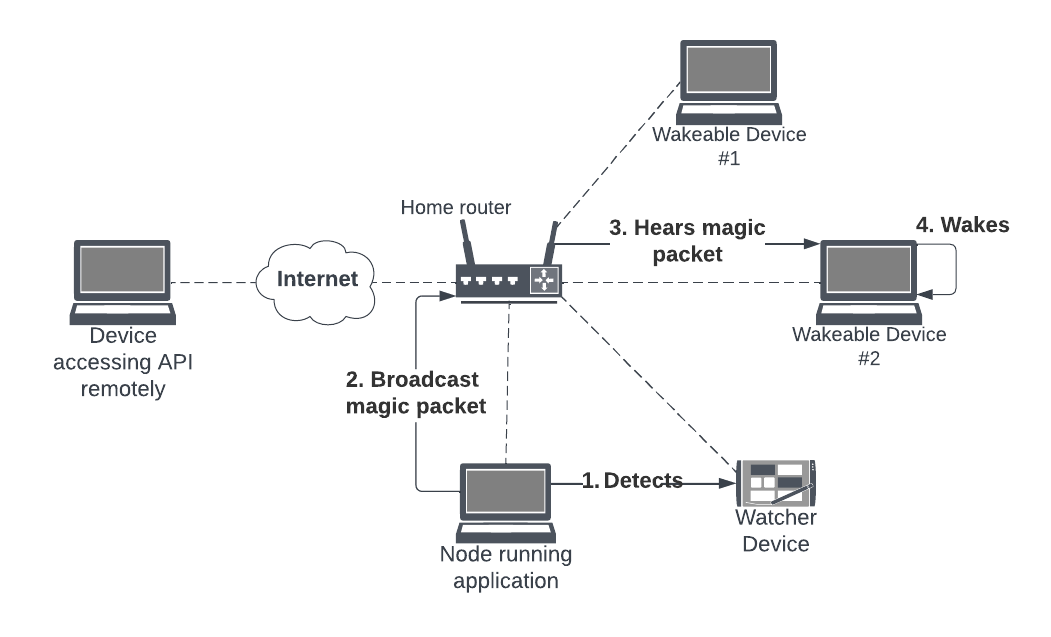
\includegraphics[width=\columnwidth]{assets/architecture.png}
    \caption{A sample architecture for the application.}
    \label{fig:architecture}
\end{figure}